%!TEX root = ../../report.tex
\chapter{Mechatronic design} % (fold)
\label{cha:design}
Designing a bipedal is a complex task that has been subdivided and analyzed in the chapter \ref{cha:analysis}.
From those results the design of RuBi can be broken down into three pieces: electronics, mechanics and software.
When designing from a holistic point of view, this three combined give a positive synergy which is the burden of this chapter.
The first of the three sections starts with the design of the electronics: from the selection of the motors based on \ref{sec:joints} and \ref{cha:mathematical_model} to the custom interfaces developed in order to reduce the weight.
Continues with the mechanical design that gathers all the constraints got from the sections \ref{sec:dimensions} and \ref{sec:physical_properties}, carries out its own mechanical analyses, like stress, durability, feasibility, design oriented to manufacturing... and concludes into a 3D model making a compromise between the requirements and manufacturability.
The last section is software, and it deals with how the control of the robot has been done.
This system is meant to be used in both the simulation and the real robot, based on ROS and with an easy interface with the already used libraries within the Maersk Mc-Kinney Møller Institute.

%!TEX root = ../../../report.tex
\section{Electronics} % (fold)
\label{sec:electronics}

%!TEX root = ../../../../report.tex

\subsection{The electric actuators} % (fold)
\label{sub:electric_actuators}
In chapter \ref{cha:mathematical_model}, the necessary characteristics of the actuators have been calculated.
In this section, the resulting theoretical requirements are used to select the final motor $+$ gearbox combination utilized.
All the documentation regarding the control of the actuators software-wise is to be found in section \ref{sec:software}.

\subsubsection{Flat BLDC Maxon motors} % (fold)
\label{ssub:the_bldc_motors}
It must be mentioned at this point that the actuators and their interface were assumed at the beginning of the project to be a very hard constraint in the design from an economic point of view. 
This means that the conception of the robot structure has been influenced by this criteria towards the adaption of the final prototype characteristics (such as final size or mass) to the application range of the available motors at our disposal.
This fact has converted the design in an iterative process of optimization whose final result is a robot that matches the available actuators and not the other way around, as it should be in theory.
In the view of the this, the brushless DC motor $+$ gearbox present in the Locokit robot construction kit, introduced in \cite{locokit} are used in the RuBi prototype.

The flat motors model is 339260 from Maxon motor, whose datasheet can be found in \cite{maxon_motor}, and the planetary gearhead is the number 143976 in datasheet \cite{maxon_gear}.
The electromechanical constants of the motors, together with its nominal supply values or the output power and torque of both the motor and the gearbox can be found in these documents. 
However, the electronics of the motors are designed to constantly overdrive them at $24V$, which has been taken into account when calculating their output.
Furthermore, each motor counts three hall effect sensors able to provide accurate relative position measurements.
% subsubsection the_bldc_motors (end)


\subsubsection{BLDC motor boards} % (fold)
\label{ssub:bldc_motor_boards}
Each BLDC motor in the Locokit comes with a motor board able to control it, designed for 24V and 48W.
They consist of a 48MHz ARM7 processor for time critical control and motor commutation, as stated in \cite{locokit-electronics}, together with 4 general purpose I/O inputs for local sensor interface.
Furthermore, they have two available 8-pin interfaces for the motors, one of them with a standard flex connector used in most of Maxon flat motors.

% subsubsection bldc_motor_boards (end)

\subsubsection{Extension PCBs} % (fold)
\label{ssub:extension_pcbs}
Following the idea of reducing weight and inertias in the structure as explained in chapter \ref{cha:analysis}, it was decided to place all the electronics off-board.
In order to extend the existing motor flex interfaces, a simple extension PCB was manufactured for each device.
The boards have been designed with Eagle following the requirements of current when sizing the width of the paths given by the supplier.
The design lacks of vias which reduces the complexity and facilitates the manufacturing.
The board for the left leg, whose schematic can be seen in \ref{fig:pcb1}\footnote{For the right leg the schematic has been mirrored}, contains a flex connector, like the one originally found on the motor boards, mapped to an 8-pin Molex connector where the wiring to the BLDC board is connected.

\begin{figure}[ht]
	\centering
	\includegraphics[width=0.5\textwidth]{figures/expansion_board.pdf}
	\caption{Left leg extension PCB schematic.}
	\label{fig:pcb1}
\end{figure}

% subsubsection extension_pcbs (end)


% subsection electric_actuators (end)
\subsection{Suitability of the motor model for the application} % (fold)
\label{sub:suitability_of_the_motor_model_for_the_application}
The algorithm designed to prove if the selected motor model fulfills the requirements of the application has been called Algorithm 1 and it is detailed in \ref{list:algorithm_1}.
The theoretical framework constructed in \ref{cha:mathematical_model} has been applied here to prove if the motors described above (without accounting on springs or indirect transmission) can be used to perform the vertical jumps described in \ref{sec:jumping_case}.
And if so, which height can be reached.

Algorithm 1:
\begin{enumerate}
\label{list:algorithm_1}
\item Manually set the values of $P_{3}(t_{0})$ and $P_{3}(t_{f})$ to use in equation \ref{eq:toe_trajectory}.
\item Compute the inverse kinematics model for the given trajectory equation. This yields as outputs $q_{j}(t)$, where j = 1,...,N being N = number of joints.
\item Compute forward kinematics to obtain $P_{j}(t)$.
\item Derive the two mentioned models and apply equation \ref{eq:angular_magnitudes} to obtain $\dot{P}_{j}$, $\ddot{P}_{j}$, $\omega_{j}$, $\omega_{j}$, $\dot{\omega}_{j}$,
\item Set $\Delta h$ and use the impulse equations \ref{eq:deltaV} and \ref{eq:impulse} to obtain a set of couple values of $(F_{i}, t_{i})$ as in Figure \ref{fig:f-t}.
\item For each couple until $(F_{min}, t_{max})$, obtained from \ref{eq:work}, compute the torques $\tau_{i,j}$ for each joint through \ref{eq:dynamics_eq1} and $\theta_{i,j}$ as in \ref{eq:joint_vel_2}\footnote{Eq. \ref{eq:joint_vel_2} introduced the assumption that the joint velocities are constant for simplicity}.
\item Compute the Torque/Speed curve for the motor + gearbox model as per equation \ref{eq:motor_curve}.
\item Plot the obtained pairs of values $(\dot{\theta}_{i,j}, \tau_{i,j})$ over the motor curve and analyze the results.
\end{enumerate}

\begin{equation}
\label{eq:joint_vel_2}
	\dot{\theta}_{i,j} =\frac{ \abs{ \theta_{j}(t_{f}) - \theta_{j}(t_{o}) } }{ t_{i} }
\end{equation}

\begin{equation}
\label{eq:motor_curve}
	\tau_{m} = \tau_{stall} - \omega_{m}\left(\frac{\tau_{stall}}{\omega_{n}}\right)
\end{equation}

\paragraph{Use case} % (fold)
\label{par:example_of_use}
As with any kind of DC motor, the goal is that the operation points lay under the torque/speed curve for a given application.
In this case, the operation point to study has been chosen to be the initial instant of the launch phase during the jump, given by $t_{0}=0s$, because it has been assumed to be the most requiring one of the whole jump cycle.
The input data for the test conducted with the algorithm can be seen in \ref{eq:input_a1}.

\begin{equation*}
\label{eq:input_a1}
\begin{aligned}[c]
P_{3}(t_{0}) &= \left[\!
				    \begin{array}{c}
				      0 \\
				      0.3508 \\
				      -\frac{\pi}{2}
				    \end{array}
				  \!\right]
\end{aligned}
\qquad
\begin{aligned}[c]
P_{3}(t_{f}) &= \left[\!
				    \begin{array}{c}
				      0 \\
				      L \\
				      0
				    \end{array}
				  \!\right]
\end{aligned}
\qquad
\begin{aligned}[c]
\Delta h &= 0.05 \\
\end{aligned}
\end{equation*}

The results can be seen in Figure \ref{fig:alg1_results} for a jumping leg.
It can be seen that, for the obtained $(\theta_{i,j}, \tau_{i,j})$ values for the given $\Delta h$, the closer they get to the theoretical $(F_{min}, t_{max})$, the more the application points approach the lower-left corner of the graph.
The aimed situation here is that in which the application points for the three motors lay under the motor curve, which occurs for values next to the couple $(4.1191N, 0.1700s)$

\begin{figure}[htb]
	\centering
	\includegraphics[width=0.9\textwidth]{figures/algorithm1.pdf}
	\caption{Results of Algorithm 1 for the given inputs (not all the $(\theta_{i,j}, \tau_{i,j})$ pairs are plotted).}
	\label{fig:alg1_results}
\end{figure}

\paragraph{The transmission on the hips} % (fold)
\label{par:the_hip_joint_gears}
The results from the presented algorithm helped notice that the presented motor model would not be able to accomplish the requirements of the application on the hip joints, due to its, in general, lower velocity and higher torque values.
Thus, the algorithm was used to approximate the required ratio of the gear system described in \ref{sub:gears}, used to adequate its output to the task.
The final ratio implemented and used for the results in \ref{fig:alg1_results} is $w=2$. 
However, it was calculated for the geometrical and inertial parameters of a different iteration than the last one, resulting in a non-optimal value for the final robot.
A repetition of the process yielded an optimal gear ratio of $w=1.2$, for which the best application points of the three motors would be closer to the motor line.

% paragraph the_hip_joint_gears (end)

The presented method does not aim at providing exact results since its based in several assumptions and simplifications from its basis.
It was conceived due to the necessity of assessing the utility of the existing actuators to the designed application.
Ideally, its results would have been tested by comparing them to the real data collected from the experimentation with the final prototype. 
However, the delay in some essential components of the robot prevented from testing and improving the model used for the algorithm, together with its validity.

% paragraph example_of_use (end)




% subsection suitability_of_the_motor_model_for_the_application (end)
%!TEX root = ../../../../report.tex

\subsection{Locokit electronics} % (fold)
\label{sub:locokit_electronics}
In chapter \ref{cha:mathematical_model}, the necessary characteristics of the actuators have been calculated.
For the sake of feasibility it was decided to utilize electric motors for supplying the power to the robot, meaning that the right model had to be selected.
It can be demonstrated from \ref{} %cite actuators section here when finished 
that the requirements of the defined application for every joint in the robot can be accomplished by the BLDC motor + gearbox present in the Locokit robot construction kit, introduced in \cite{locokit}.
The flat motors model is 339260 from Maxon motor, whose datasheet can be found in \cite{maxon_motor}, and the planetary gearhead is the number 143976 in datasheet \cite{maxon_gear}.

% subsection locokit_electronics (end)
%!TEX root = ../../../../report.tex

\subsection{Sensory feedback} % (fold)
\label{sub:sensory_feedback}
As stated in the initial description of the project in \ref{sec:overall_description}, the first prototype of RuBi has been designed to provide the necessary capabilities to be controlled by an existing neural controller developed in \cite{dacbot1} and already tested in the DACbot robot.
The cited control algorithm requires as inputs the angular positions of all the joints in can actuate, besides ground contact signals from the feet for its reflex-based controller part.
All the documentation regarding the handling of the sensor readings software-wise is to be found in section \ref{sec:software}.


\subsubsection{Joint position information} % (fold)
\label{ssub:joint_position_feedback}
To provide the physical readings of the angular positions of the joints, the built-in hall sensors in the motors are utilized. 
Three wires transmit the hall effect sensors signals to the motor board for each joint, where they are written in the internal register and transferred to the main processor for its posterior treatment.
% subsubsection joint_position_feedback (end)

\subsubsection{Ground contact signal} % (fold)
\label{ssub:ground_contact_feedback}
One contact switch model Omron D2F-01F-T has been placed on the edge of the sole of each foot, under the heel in order to detect when the feet are standing on the ground. 
Their wiring has been extended to the main processor board, but the necessary pull-up resistors have not been implemented since the input pins on the processor could not be set up.
The mapping between the processor's GPIOS handlers and the physical pins on the board could not be found.
Therefore this last step is left as further work.
Alternatives to the use of the main board pins are discussed in chapter \ref{cha:discussion}, in case they cannot be used.
% subsubsection ground_contact_feedback (end)

% subsection sensory_feedback (end)

% section electronics (end)
%!TEX root = ../../../report.tex
\section{Mechanics} % (fold)
\label{sec:mechanics}
This section deals with the mechanical design of the robot.
Based on the analysis performed in the chapter \ref{cha:analysis}, the mechancal design takes its results and carries out a specific analysis of each component.
Then, the conclusions are translated into a 3D model making a compromise between the requirements and manufacturability.

%!TEX root = ../../../../report.tex
\subsection{Motion transmission} % (fold)
\todo{Include a new section(?) detailing the implementation of the DD, SEA, PEA and SEA+PEA options}
\label{sub:pulleys_and_belts}
The section \ref{sec:joints} is dedicated to analyze and define what kind of motors and trasmision system is going to be used for each joint.
In the case of the knee and the ankle, the combination \textit{motor + gearbox + belt and pulleys} is chosen due to the preference of having the active actuator in the highest part of the link with the withdrawal of having to transfer the movement the lowest.
This system has been designed along with the torsional springs disussed in the section \ref{sub:compliance} where the rotation from the motor must feed the rotation of a serial rotational spring.
A system in which pulley and spring holder are joined, have to be done then.
The design of the pulley itself though, has been studied in terms of two factors: \textit{precision and backlash reduction} and \textit{integration with the serial rotational spring}.

\subsubsection{Precision and backlash reduction} % (fold)
\label{ssub:precision_and_backlash_reduction}
The goal of this design is to optimize the pulley in order to to get a lack of backlash.
Despite the platform is going to be used mainly for self-learning controllers (e.g. based on neuronal networks) and then the mechanical optimization is not a priority, the reduction of mechanical uncertainty is always good.

After analyze all the current solutions in the market, several non-backlash solutions are found.
Stands out the Gates GT3 Synchronous Belts \footnote{http://www.gates.com/products/industrial/industrial-belts/synchronous-belts/powergrip-gt3-belts} that is assured to be suitable for the presented application.
The withdrawals of this design are the lack of time for ordering such parts and the increase in the final price of the product. 
However there is another important factor, the integration that must be done with the serial rotational spring.
% subsubsection precision_and_backlash_reduction (end)

\subsubsection{Integration with the serial rotational spring} % (fold)
\label{ssub:integration_with_the_serial_rotational}
Another solution is to design and manufacture the pulley itself which would let to have a complete control of the design and manufacturability giving the possibility of integrate in a unique part design, the pulley for the transmission system and the spring holder.

At first, the GT3 design from Gates was intended to be designed.
However, its design is described in U.S. Patent Number 4,515,577, which doesn't allow its use.
Thus, the belts have been designed following the ISO 13050:2014 \cite{ISO13050} following the type T due to its focus in efficiency and reduction of backlash.
It is also appropriate for precision movements, high torques and low speeds, as our requirements.

The physical properties of the pulleys as the number of teeth, width, etc... have been chosen based on the ISO 5295:1987 \cite{ISO5295} and in sake of manufacturability.
As decided before, the pulley will belong to a part that will also have the task of holding the rotational serial spring.
This implies that the part will be designed to be 3D printed and thus, the criteria of design oriented to manufacturability must be applied.

Based on both ISO norms cited before and after some iterations based on experimental tests, the pulley T2,5 of 19 teeth gave the expected behavior.
Both pulleys are the same so no reduction is given from the motor shaft to he other.
In the figure \ref{fig:motor_pulley}, a detail of the designed pulleys can be seen.
% subsubsection integration_with_the_serial_rotational (end)

\subsubsection{Belts} % (fold)
\label{ssub:belts}
From \ref{ssub:integration_with_the_serial_rotational} a system pulleys-belt using T2,5 teeth profile was selected.
For the design of the belt system, an open belt whose initial tension can be adjusted with a zip-tie is chosen.
This allows to adjust the tension in any moment without increasing the costs plus it easy the maintenance.
No initial tensioning of the belts studies were carried out and it is expected that the user finds out the correct value by experimenting.
% subsubsection belts (end)

% subsection pulleys_and_belts (end)
%!TEX root = ../../../../report.tex
\subsection{Gears} % (fold)
\label{sub:gears}

\begin{figure}[ht!]
  \centering
  \includegraphics[width=0.5\textwidth]{figures/hip_gears}
  \caption{Teeth detail from pinion and gear.}
  \label{fig:teeth_detail}
\end{figure}

% subsection gears (end)
%!TEX root = ../../../../report.tex
\subsection{Impact force} % (fold)
\label{sub:impact_force}
In order to calculate the physical dimensions of some of the components, a bounding conditions have to be defined.
The presented case shows a peak of energy when landing after being jumped a estimated height.
This energy in then transmitted from the first contact point, the footprint, to the rest of the system, causing efforts that must be absorbed.
The components of the system must receive that energy under a controlled behavior -this is elastic deformations- assuring a longer life cycle of the legs.

Thus, some input parameters to calculate the impact force are assumed.
From this force will be sized all the consecutive components in the deformation chain.
Despite the deformation is of the whole system, the security coefficient assumed in here is going to be the calculation of all the components for that maximum force.

From the formula of the mechanical energy:
\begin{equation}
  E_{mechanical} = m g \Delta h + \frac{1}{2} m v^{2}
\end{equation}

The kinetic energy is negligible and only the energy form falling a certain height is supposed.
This energy is then translated into force by supposing a deformation of the whole body:
\begin{equation}
\label{eq:impact_force}
  F_{impact} = \frac{m g \Delta h}{t_{impact\_displacement}}
\end{equation}

The equation \ref{eq:impact_force} gives the force for sizing all the components.
Based on the input parameters defined in the appendix \ref{app:profile_selection} which are:
\begin{center}
\begin{tabular}{c | c}
  Parameter & Value \\
  \hline
  Total mass [kg] & 1.5 \\
  Jumping height [m] & 0.1 \\
  Impact displacement [m] & 0.005
\end{tabular}
\end{center}

The impact force is thus:
\begin{equation}
  F_{impact} = \frac{m g \Delta h}{t_{impact\_displacement}} = 294.40 N 
\end{equation}
% subsection impact_force (end)
%!TEX root = ../../../../report.tex
\subsection{Limb profile} % (fold)
\label{sub:limb_profile}
Based on the requirements of weight and its distribution defined in the analysis of the joints \ref{sec:joints}, the links have been decided to have in the upper extreme the motors. 
This leads to use a transmission system, such as belt and pulleys, which leaves for the rest of link an structural function that can also adopt the task of wiring placement.

Thus, a light weight section that satisfy the conditions of deformation and stress maximum will be chosen.
Carbon fiber is an ideal material to achieve this conditions of weight and stress so an quantitative analysis has been made calculating the optimal solution and then rounding it for all the possible profiles offered by the given provider.
The provider was chosen due to the previous experiences that the Mærsk Mc-Kinney Møller Institute had with carbon fiber orders.

The section profile offered \footnote{http://www.easycomposites.co.uk/\#!/cured-carbon-fibre-products/} are: \textit{Rod}, \textit{Tube}, \textit{Box}. The \textit{Stripe} and the \textit{Angle} are discarded due to its asymmetrical geometry that will will lead to less predictable scenarios.

  \subsubsection{subsubsection name} % (fold)
  \label{ssub:subsubsection_name}
  
  % subsubsection subsubsection_name (end)



% subsection limb_profile (end) 
%!TEX root = ../../../../report.tex

\subsection{Bearings} % (fold)
\label{sub:bearings}
In the section \ref{sub:impact_force} the force for sizing the bearings of the knee and the ankle was calculated.
The bearing elected would be such that allow dynamic loads of more than the impact force while keeping as small as possible to reduce the added weight to the robot.
On the other hand, the internal diameter comes defines by the rod diameter calculated in the section \ref{sub:rods}.

An estimation of nominal life of the bearing can be done from the Dynamic Load Rating (C), the Dynamic Equivalent Load (P) and the Life Rime Coefficient for a Ball Bearing (p) (being p=3 for balls bearings).
The equation \ref{eq:service_life_bearing}, shows the nominal life of one selected bearing \footnote{http://dk.rs-online.com/web/p/kuglelejer/8937420/}.
It is also worth to mention that the Dynamic Equivalent Load (P) is divided by the number of bearings in which the force is spread.
\begin{equation}
  \label{eq:service_life_bearing}
  L_{10} = \frac{10^{6}}{60 n} \left(\frac{C}{P}\right)^{p} = \frac{10^{6}}{60 n} \left(\frac{403}{294.4}\right)^{3} = 
\end{equation}

The term $L$ is the service life of a bearing (in number of hours or rpm), in normal conditions of speed and load, in which the bearing is working until fail by fatigue. 
Whilst $L_{10}$ is based in a stadistical model that is defined as the 90\% of the bearing of the same type will withstand those loads for a longer time.
% subsection bearings (end)
%!TEX root = ../../../../report.tex
\subsection{Rods} % (fold)
\label{sub:rods}
As explained in section \ref{sub:bearings}, it was decided to have two bearings per link (which gives four per joint) and a rod going through them.
This rod is then also used, in the case of the knee and the ankle, as a support for the pulleys that transmit the power from the motor to the next link.

Three mechanical efforts bound its design:
\begin{enumerate}
  \item \textbf{Shear strength}: in the case of the shear produced when an impact occurs and the rod of one link moves in the opposite direction than its relative in the consecutive link.
  \item \textbf{Resistance to bending}: due to the bending effort that the tension of the belt is constantly applying in the rod of the  knee and the ankle.
  \item \textbf{Torsion}: due to the pulley in the knee and the ankle. 
  This effort is negligible because zero-friction bearings are supposed.
\end{enumerate}

  \subsubsection{Shear analysis} % (fold)
  \label{ssub:shear_analysis}
  The maximum shear stress is found in the diameter of the cylinder (y=0) and is:
  
  \noindent\begin{minipage}{0.2\textwidth}% adapt widths of minipages to your needs
  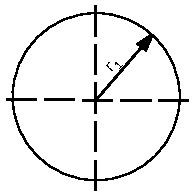
\includegraphics[width=\linewidth]{figures/profile_tube.pdf}
  \end{minipage}%
  \hfill%
  \begin{minipage}{0.8\textwidth}
    \begin{equation}
    \begin{aligned}
      \gamma_{yz} &= \frac{Q_y M_{x}^A*}{b(y) I_x} = \frac{Q}{r^2}\\
      M_{x}^{A_{y=0}} &= \frac{\pi r_1^2}{2} \\
      b(y=0) &= 2 r_1 \\
      I_x &= \frac{\pi r_1^4}{4}
      \end{aligned}
    \end{equation}
  \end{minipage}
  Given a tangent force Q, the shear stress can be calculated.
  If this is over the ultimate strength, the cylinder will break.
  % subsubsection shear_analysis (end)

  \subsubsection{Bending} % (fold)
  \label{ssub:bending}
  The bending analysis follows the one carried out in the section \ref{ssub:profile_study} for a cylinder.
  The equivalent force in this case is given by the tension of the belts, mainly the initial (though there are other tensions that appear when the belts moves for example).
  Due to feasibility reasons and the lack of the appropriate measurements devices, some experimental tests trying different tensions and axes where carried out giving good results with a 3 mm rod or more.
  % subsubsection bending (end)

  \subsubsection{Sizing} % (fold)
  \label{ssub:sizing}
  The studies above have been tested for different diameters of rod starting from the smallest size given by the provider and increasing until both conditions are satisfied, due to the requirements of weight reduction.
  In case of using steel as material, the ultimate strength is supposed to be 250 MPa\footnote{https://en.wikipedia.org/wiki/A36\_steel}.
  And for the case of a rod of 3 mm of diameter, both stresses are under the restrictions.
  Thus, 3 mm rods are going to be used.
  % subsubsection sizing (end)
% section rods (end)
%!TEX root = ../../../../report.tex

\subsection{Finite Element Method (FEM)} % (fold)
\label{sub:finite_element_method}
In the sections \ref{sub:limb_profile} and \ref{sub:rods}, pure mathematical tools have been used to calculate deformations and stresses.
This has been possible due to the simplification of the problem and the simple geometries found.
However, other parts have been analyzed with Finite Element Analysis (FEM), in which the part is subdivided into small volumes and then analyzed individually.
This allows the deformation and stress studies of complex geometries.

As an example, in the figures \ref{fig:fem_foot_iteration_1} and \ref{fig:fem_foot_iteration_2}, the iterative foot design is depicted.
Once the first iteration of the foot was modeled, the design has been changed in order to satisfy a minimum deformation criteria.
However, the designs have always been tested experimentally due to this analysis are under the assumption of isomorphic materials which, in the case of 3D printed parts like the shown in the figures, is not true.
The FEM studies have been used more as a qualitative analysis rather than quantitative.

\begin{figure}[ht]
    \centering
    \begin{subfigure}[b]{0.49\textwidth}
        \includegraphics[width=\textwidth]{figures/fem_5N_1.PNG}
        \caption{FEM analysis in left foot iteration 1}
        \label{fig:fem_foot_iteration_1}
    \end{subfigure}
    \begin{subfigure}[b]{0.49\textwidth}
        \includegraphics[width=\textwidth]{figures/fem_5N_2.PNG}
        \caption{FEM analysis in left foot iteration 2}
        \label{fig:fem_foot_iteration_2}
    \end{subfigure}
\end{figure}

% subsection finite_element_method (end)
%!TEX root = ../../../../report.tex
\subsection{Computer-Aided Design (CAD)} % (fold)
\label{sub:computer_aided_design}

\begin{figure}
    \centering
    \begin{subfigure}[b]{0.49\textwidth}
        \includegraphics[width=\textwidth]{figures/legs_foot.jpg}
        \caption{Left foot}
        \label{fig:left_foot}
    \end{subfigure}
    \begin{subfigure}[b]{0.49\textwidth}
        \includegraphics[width=\textwidth]{figures/legs_hip.jpg}
        \caption{Hip}
        \label{fig:hip}
    \end{subfigure}

    \begin{subfigure}[b]{0.49\textwidth}
        \includegraphics[width=\textwidth]{figures/legs_parts.jpg}
        \caption{Additional designed parts}
        \label{fig:mouse}
    \end{subfigure}
    \begin{subfigure}[b]{0.49\textwidth}
        \includegraphics[width=\textwidth]{figures/legs_pulley.jpg}
        \caption{Left ankle serial spring pulley}
        \label{fig:serial_spring_pulley}
    \end{subfigure}

    \begin{subfigure}[b]{0.49\textwidth}
        \includegraphics[width=\textwidth]{figures/legs_pulley_motor.jpg}
        \caption{Motor pulley}
        \label{fig:motor_pulley}
    \end{subfigure}
    \begin{subfigure}[b]{0.49\textwidth}
        \includegraphics[width=\textwidth]{figures/legs_knee_lower.jpg}
        \caption{Left lower knee}
        \label{fig:lower_knee}
    \end{subfigure}

    \begin{subfigure}[b]{0.49\textwidth}
        \includegraphics[width=\textwidth]{figures/legs_ankle_upper.jpg}
        \caption{Left upper ankle}
        \label{fig:ankle_upper}
    \end{subfigure}
    \begin{subfigure}[b]{0.49\textwidth}
        \includegraphics[width=\textwidth]{figures/legs_hip_lower.jpg}
        \caption{Left lower hip}
        \label{fig:hip_lower}
    \end{subfigure}

    \begin{subfigure}[b]{0.49\textwidth}
        \includegraphics[width=\textwidth]{figures/legs_hip_pinion.jpg}
        \caption{Hip's pinion}
        \label{fig:hip_pinion}
    \end{subfigure}
    \begin{subfigure}[b]{0.49\textwidth}
        \includegraphics[width=\textwidth]{figures/legs_knee_upper.jpg}
        \caption{Left upper knee}
        \label{fig:knee_upper}
    \end{subfigure}
\end{figure}

% subsection computer_aided_design (end)
%!TEX root = ../../../../report.tex
\subsection{Mechanical limits of the joints} % (fold)
\label{sub:mechanical_limits}
The implementation of mechanical limits for the joints obeys to two reasons:
\begin{enumerate}
  \item \textbf{Calibration}: they can be used as starting, known positions for the relative encoders.
  \item \textbf{Security}: a mechanical limit will restrict the movements and prevent any configuration non-natural or dangerous for the physical integrity of the robot.
\end{enumerate}

The Figure \ref{fig:joint_limits_hip} depicts how the mechanical limits of the hip (both left and right) are implemented in the upper part, comprising an angle of 90 + 60 = 150 degrees.
Figure \ref{fig:joint_limits_ankle_upper} shows the upper part of the ankle and how the allowed movement of the foot has a range of 60 + 50 = 110 degrees.
The mechanical limits of the knee are obtained as a combination of the lower and upper components of the joint.
These allow movements of 0 + 120 = 120 degrees as shown in the figures \ref{fig:joint_limits_knee_upper} and \ref{fig:joint_limits_knee_lower}.
The angles of the mechanical limits have been calculated according to the physical limitations in humans.

\begin{figure}[ht!]
    \centering
    \begin{subfigure}[b]{0.49\textwidth}
        \includegraphics[width=\textwidth]{figures/joint_limits_hip.PNG}
        \caption{Joint limits of the hip}
        \label{fig:joint_limits_hip}
    \end{subfigure}
    \begin{subfigure}[b]{0.49\textwidth}
        \includegraphics[width=\textwidth]{figures/joint_limits_ankle_upper.PNG}
        \caption{Joint limits of the ankle}
        \label{fig:joint_limits_ankle_upper}
    \end{subfigure}
\end{figure}    

\begin{figure}[ht!]
    \ContinuedFloat % continue from previous page
    \begin{subfigure}[b]{0.49\textwidth}
        \includegraphics[width=\textwidth]{figures/joint_limits_knee_upper.PNG}
        \caption{Joint limits of the knee: Upper link}
        \label{fig:joint_limits_knee_upper}
    \end{subfigure}
    \begin{subfigure}[b]{0.49\textwidth}
        \includegraphics[width=\textwidth]{figures/joint_limits_knee_lower.PNG}
        \caption{Joint limits of the knee: Lower link}
        \label{fig:joint_limits_knee_lower}
    \end{subfigure}
\end{figure}    

% subsection mechanical_limits (end)

% section mechanics (end)
%!TEX root = ../../../report.tex
\vfill
\section{Software} % (fold)
\label{sec:software}

%!TEX root = ../../../../report.tex

\subsection{Motivation} % (fold)
\label{sub:motivation}
When approaching the task of designing a new robotic platform for the AI department at the Mærsk Mc-Kinney Møller Institute, the current development environment being utilized and its capabilities were studied as a first step.
Nowadays, the simulation and control of the robots at the department is based on the LPZrobots \cite{lpzrobots} and Gorobots \cite{gorobots} packages.
These software tools provide both a simulation engine for robots built on ODE \cite{ode}, OSG \cite{osg} and a framework for an easy implementation of controllers in both simulation and hardware.
However, their specificity compared to other existing instruments collides with some of the core design ideas of the robot framework presented here, which are simplicity of use and generalization.
The above mentioned are the reasons why it was decided to migrate the development environment to ROS Jade \cite{ros} for the bipedal locomotion study framework of RuBy. 

% subsection motivation (end)
%!TEX root = ../../../../report.tex

\subsection{ROS control} % (fold)
\label{sub:ros_control}

% subsection ros_control (end)
%!TEX root = ../../../../report.tex
\subsection{ROS control-locokit hardware interface} % (fold)
\label{sub:ros_control_hardware_locokit_interface}

%initialization of enconders for sensory feedback!

% subsection ros_control_hardware_locokit_interface (end)
%!TEX root = ../../../../report.tex

\subsection{Example controllers} % (fold)
\label{sub:example_controllers}
From the \textit{Controller manager} from ROS Control, different joint controllers can be handled.
In the example controllers the position controller and the effort controllers are used individually for each joint.
This joint controllers offer then a topic (e.g. /rubi/left\_ankle\_position) that the user can use to move the actuators.
This are created from a unique package called \textit{rubi\_joint\_controllers}.
It is worth to say that the position controllers are implemented with a PID and that these values have been adjusted experimentally with the simulations for each joint.

Two type of controllers are given that show a different range of options to use with the robot.
Both are gathered in a sole package called \textit{rubi\_controllers}, which gives a more tidy and resource-shared environment rather than having a package for each controller.
This also makes really easy the deployment a new controller by removing all the creation process of a new package.
In order to start a new piece of code this must be created and then added in the \textit{CMakeLists.txt} from where also some examples are included.

The presented code follows the ROS conventions and the code style is the \textit{Google style} offered by the clang-code-model.
This creates a congruent workspace supervised by a git repository.

\subsubsection{Two neuron controller} % (fold)
\label{ssub:two_neuron_controller}
This first example controller shows how to:
\begin{enumerate}
    \item Use GoRobots.
    \item Make use of dynamic reconfigure.
    \item Adapts its behavior depending on gazebo real time factor.
\end{enumerate}
For the first, an example of how to link C++ code from GoRobots is shown in the \textit{CMakeLists.txt}.
This system is easier and more powerful than the current \textit{Makefiles} currently used in GoRobots.
The Artificial Neuronal Network (ANN) library is used to create a bi-neuronal network that creates the CPG signals of the actuators.
Furthermore, the synaptic weights can be modified by making use of the ROS feature \textit{Dynamic Reconfigurable Parameters}.
These offer an interface in order to change, on the fly, the the values of the created parameters.
In the Figure \ref{fig:rqt_interface}, an RQT workspace containing the CPG signals and the dynamic reconfigurable parameters modifiers is depicted.

\begin{figure}[tb]
    \centering
    \includegraphics[width=\textwidth]{figures/rqt_interface}
    \caption{RQT workspace containing the CPG signals and the dynamic recofigurable parameters.}
    \label{fig:rqt_interface}
\end{figure}

This are also used to change the behavior of the ANN in order to be adapted to changes in Gazebo.
Gazebo uses can accelerate and decelerate the speed at which the time is passing through.
This is adjusted with a \textit{real time factor} that is read by the node and used to adjust the frequencies of the CPGs.
% subsubsection two_neuron_controller (end)

\subsubsection{Impulse controller} % (fold)
\label{ssub:impulse_controller}
Among other things this node shows how to:
\begin{enumerate}
    \item Load and unload different joint controllers.
    \item Give some wrappings for set of controllers (hoping position).
    \item Offer services for jumping: given a file or given the values and impulse time.
\end{enumerate}
This node implements some methods that enable it to change on-the-fly the controllers of each individual joint.
Furthermore, three combinations of individual joint controllers are given being these: (1) all in position mode, (2) all in effort mode and (3) left leg in position mode and right in effort mode.
The last one is useful when hoping, a moment in which a leg must hold a position and the other keep pushing in order to jump.

Three different services are implemented that impulse the robot in the sake of rise it from the floor.
The first two, are \textit{impulse\_one\_leg} and \textit{impulse\_two\_legs} which given a torque for each joint and an impulse time, it gives the possibility to jump either with one or two legs.
Both services load the necessary joint controllers in order to achieve the desired movements.
The third one offers sort of the same service but the parameters are read from a file instead.
This is handy when combined with the dynamic controller developed in MatLab and explained in the section \ref{sec_dynamic_model}.
% subsubsection impulse_controller (end)

% subsection example_controllers (end)

% section software (end)

% chapter design (end)chapters/cha_design/